\documentclass[usenames,dvipsnames,tikz]{standalone}
\usepackage{amsmath,amssymb}
\usepackage{xcolor}
\colorlet{tBlue}{RoyalBlue!35!Cerulean}
\colorlet{tRed}{Red}
\usepackage{tikz}
\usepackage{standalone}
\begin{document}
	
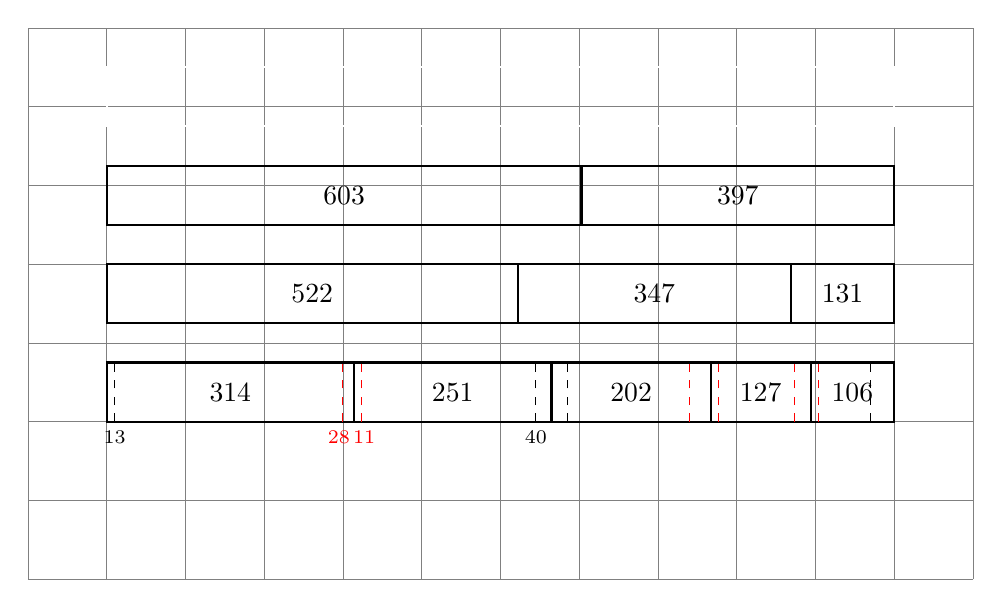
\begin{tikzpicture}
\draw [help lines] (-1,-2) grid (11,5);
% 1=0.1, 2=0.15, 3=0.2, 4=0.25, 5=0.3
% 6 (3-27), 5 (8-42), 4 (33-65), 4 (16-22), 3 (13-28), 3 (11-40), 2 (35-50), 1 (15-30), 1 (14-38), 1 (4-57).

% BPP
\draw [thick] (0,0) rectangle (10,0.75);
\draw [thick] (0,1.25) rectangle (10,2);
\draw [thick] (0,2.5) rectangle (10,3.25);
\draw [thick, white] (0,3.75) rectangle (10,4.5);
 
% Bottom row, 314, 251, 202, 127, 106 (13-28 X 11-40, 35-50 X 14-38 X 4-47)
\draw [thick] (3.14,0) -- (3.14,0.75);
\draw [thick] (5.65,0) -- (5.65,0.75);
\draw [thick] (7.67,0) -- (7.67,0.75);
\draw [thick] (8.94,0) -- (8.94,0.75);

\draw [dashed] (0.1,0) -- (0.1,0.75); 
\draw [dashed, tRed] (3,0) -- (3,0.75);
\node [below] at (0.1,0) {\scriptsize{13}};
\node [below] at (2.95,0) {\textcolor{tRed}{\scriptsize{28}}};

\draw [dashed, tRed] (3.24,0) -- (3.24,0.75);
\draw [dashed] (5.45,0) -- (5.45,0.75);
\node [below] at (3.27,0) {\textcolor{tRed}{\scriptsize{11}}};
\node [below] at (5.45,0) {\scriptsize{40}};

\draw [dashed] (5.85,0) -- (5.85,0.75);
\draw [dashed, tRed] (7.4,0) -- (7.4,0.75);
%\node [below] at (4.8,0) {\scriptsize{35}};
%\node [below] at (5.65,0) {\textcolor{tRed}{\scriptsize{50}}};

\draw [dashed, tRed] (7.77,0) -- (7.77,0.75);
\draw [dashed, tRed] (8.74,0) -- (8.74,0.75);
%\node [below] at (6.1,0) {\textcolor{tRed}{\scriptsize{14}}};
%\node [below] at (6.5,0) {\textcolor{tRed}{\scriptsize{38}}};

\draw [dashed, tRed] (9.04,0) -- (9.04,0.75);
\draw [dashed] (9.7,0) -- (9.7,0.75);
%\node [below] at (6.85,0) {\textcolor{tRed}{\scriptsize{4}}};
%\node [below] at (7.2,0) {\scriptsize{57}};

\node at (1.57, 0.375) {314};
\node at (4.395, 0.375) {251};
\node at (6.66, 0.375) {202};
\node at (8.305, 0.375) {127};
\node at (9.47, 0.375) {106};

% Middle row, 522, 347, 131 (8-42 X 16-22 X 15-30)
\draw [thick] (5.22,1.25) -- (5.22,2);
\draw [thick] (8.69,1.25) -- (8.69,2);
%\draw [dashed] (0.1,1.25) -- (0.1,2);
%\draw [dashed, tRed] (3.45,1.25) -- (3.45,2);
%\draw [dashed, tRed] (3.95,1.25) -- (3.95,2);
%\draw [dashed, tRed] (6.55,1.25) -- (6.55,2);
%\draw [dashed, tRed] (6.95,1.25) -- (6.95,2);
%\draw [dashed] (7.25,1.25) -- (7.25,2);
%\node [below] at (0.1,1.25) {\scriptsize{8}};
%\node [below] at (3.45,1.25) {\textcolor{tRed}{\scriptsize{42}}};
%\node [below] at (3.95,1.25) {\textcolor{tRed}{\scriptsize{16}}};
%\node [below] at (6.55,1.25) {\textcolor{tRed}{\scriptsize{22}}};
%\node [below] at (6.9,1.25) {\textcolor{tRed}{\scriptsize{15}}};
%\node [below] at (7.25,1.25) {\scriptsize{30}};
\node at (2.61, 1.625) {522};
\node at (6.955, 1.625) {347};
\node at (9.345, 1.625) {131};

% Top row, 603, 397 (3-27 X 33-65)
\draw [thick] (6.03,2.5) -- (6.03,3.25);
%\draw [dashed] (0.1,2.5) -- (0.1,3.25);
%\draw [dashed, tRed] (4.25,2.5) -- (4.25,3.25);
%\draw [dashed, tRed] (4.75,2.5) -- (4.75,3.25);
%\draw [dashed] (7.05,2.5) -- (7.05,3.25);
%\node [below] at (0.1,2.5) {\scriptsize{3}};
%\node [below] at (4.25,2.5) {\textcolor{tRed}{\scriptsize{27}}};
%\node [below] at (4.75,2.5) {\textcolor{tRed}{\scriptsize{33}}};
%\node [below] at (7.05,2.5) {\scriptsize{65}};
\node at (3.015, 2.875) {603};
\node at (8.015, 2.875) {397};


\end{tikzpicture}

\end{document}